Im Versuch wurde der Frequenzgang der Tiefpassschaltung mit dem Oszilloskop
durch Messung der Effektivwerte der Ausgangsspannungen bei konstanter
Eingangsspannung (Sinusförmig $U_{\mathrm{eff}} \approx 950 \,
\si{\milli\volt}$) sowie der Phasenverschiebung ermittelt.

Die Gleichspannungsverstärkung sollte auf den Wert 5 bei gegebenen Widerstand
$R_1$ eingestellt werden. Der Widerstandswert $R_2$ in der Gegenkopplung ist daher
\[R_2 = |V(\omega=0)| \cdot R_1 = 5 \cdot 1\, \si{\kilo\ohm} = 5 \, \si{\kilo\ohm}\]
% Please add the following required packages to your document preamble:
% \usepackage{booktabs}
% \usepackage[table,xcdraw]{xcolor}
% If you use beamer only pass "xcolor=table" option, i.e. \documentclass[xcolor=table]{beamer}

\begin{table}[H]
  \begin{center}
\begin{tabular}{@{}lll@{}}
\toprule
$f / \si{\hertz}$ & $U_{\mathrm{a, eff}} / \si{\volt}$ & $\phi / \si{\degree}$ \\ \midrule
20                & 4.728                              & 174.56               \\
100               & 4.526                              & 161.7                \\
250               & 3.756                              & 140.52               \\
280               & 3.589                              & 137                  \\
\rowcolor{gray1} 
300               & 3.484                              & 137                  \\
\rowcolor{gray1} 
320               & 3.377                              & 134.5                \\
\rowcolor{gray1} 
340               & 3.272                              & 131.8                \\
400               & 2.991                              & 127                  \\
500               & 2.585                              & 120.5                \\
750               & 1.888                              & 111.6                \\
1000              & 1.471                              & 105.5                \\
2000              & 0.77010                             & 96.5                 \\
3000              & 0.51890                             & 93.1                 \\
4000              & 0.39030                             & 95.7                 \\
5000              & 0.31340                             & 91.4                 \\
6000              & 0.25802                            & 91.5                 \\
7000              & 0.22158                            & 89.9                 \\
8000              & 0.19423                            & 90.3                 \\
9000              & 0.17300                              & 88.6                 \\
10000             & 0.15599                            & 91.3                 \\ \bottomrule
\end{tabular}
\end{center}
\caption{Messwerte des Tiefpassfrequenzganges}
\end{table}

\subsubsection{Betragsgang}

\begin{figure}[H]
\begin{center}
  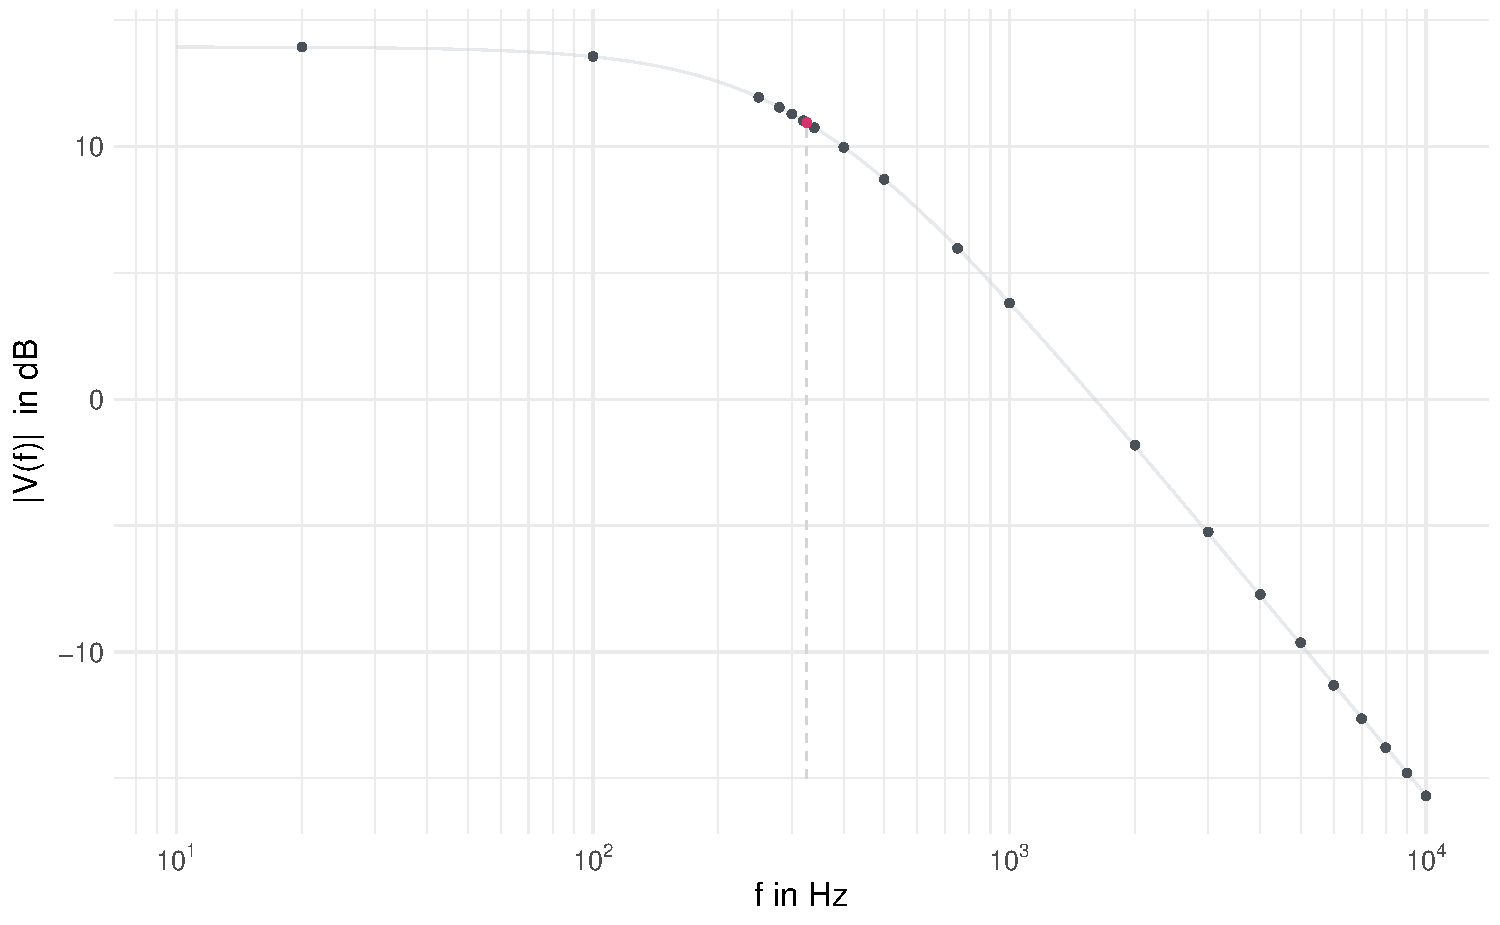
\includegraphics[width=\textwidth]{/VERA/5_5/frequenzgang_TP}
\end{center}
\caption{Verstärkungswerte der Tiefpassschaltung im Bode-Diagramm}
\label{fig:tpverst}
\end{figure}

In Abb. \ref{fig:tpverst} sind die Messwerte der Verstärkungen ($U_a / U_e$)
in $\si{\deci\bel}$ der
Tiefpassschaltung im Bode-Diagramm dargestellt. Die Grenzfrequenz der Schaltung wurde mithilfe der
Regressionsfunktion bei einem Abfall um $3\, \si{\deci\bel}$ ermittelt.
\[f_g = 326.16 \, \si{\hertz}\]

Der Anstieg der Asymptote nach der Grenzfrequenz ist etwa $-19.5 \,
\si{\deci\bel}/\mathrm{dek}$, kommt also sehr nahe an den eines Tiefpasses
erster Ordnung ($-20\,\si{\deci\bel}/\textrm{dek}$) heran.

\subsubsection{Phasengang}
\begin{figure}[H]
\begin{center}
  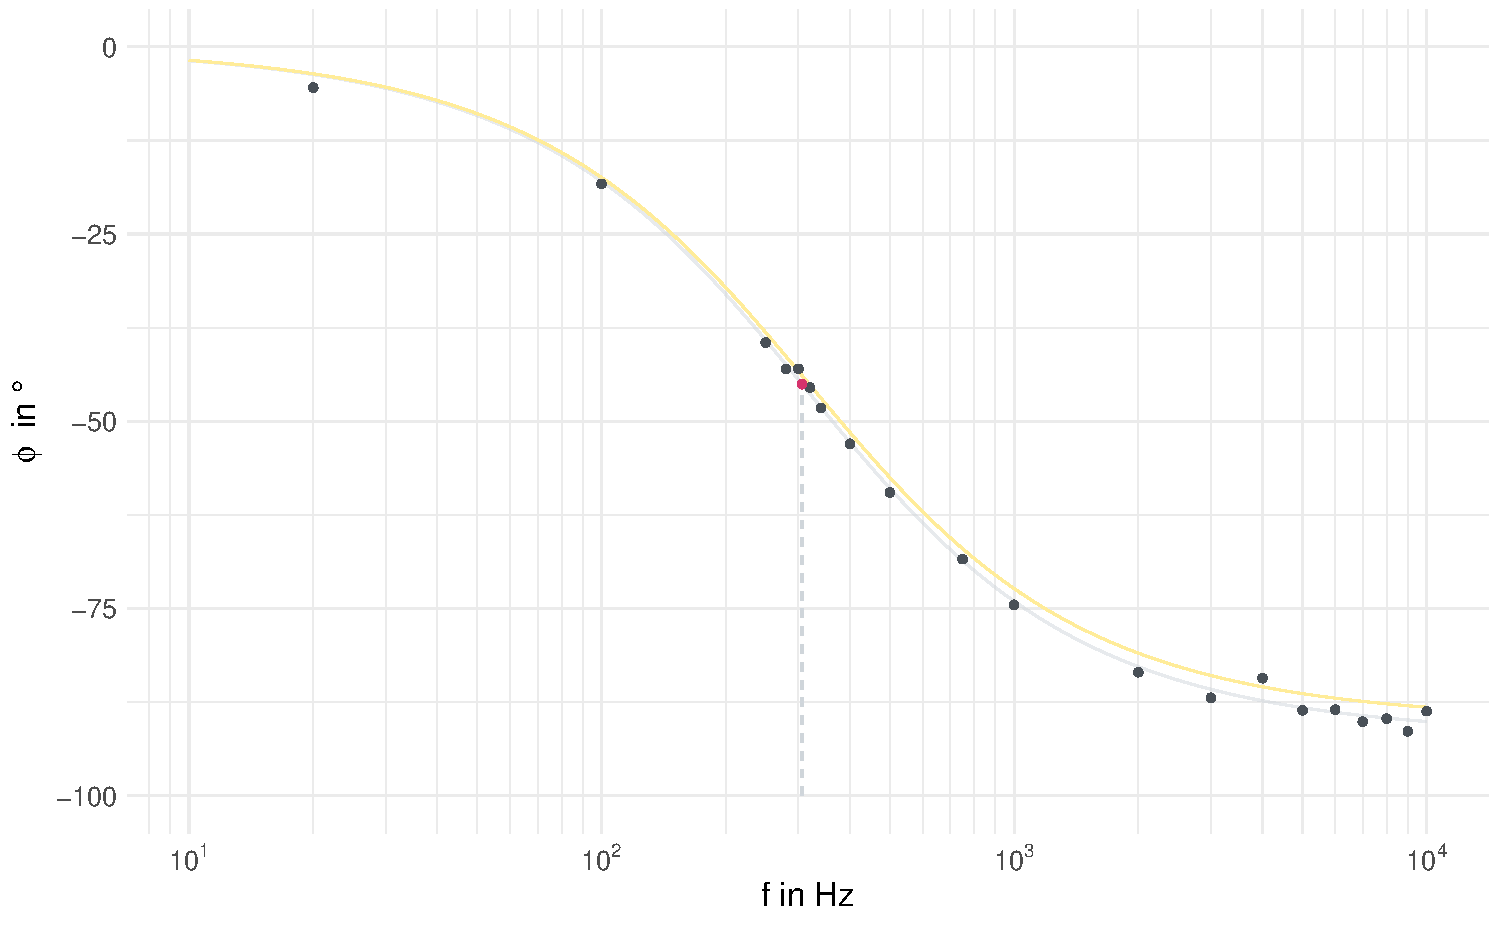
\includegraphics[width=\textwidth]{/VERA/5_5/phasengang_TP}
\end{center}
\caption{Phasenverschiebung der Tiefpassschaltung über der Frequenz, gelb zeigt
  den theoretischen Verlauf ($\tau = 500 \, \si{\micro\second}$), grau die Regressionsfunktion}
\label{fig:tpphase}
\end{figure}

In Abb. \ref{fig:tpphase} sind die Phasenmesswerte der Tiefpassschaltung über der
Frequenz dargestellt. Dabei wurde die Grundphasendrehung um
$180 \, \si{\degree}$ durch die invertierende Schaltungscharakteristik berücksichtigt.
Die hieraus ermittelte Grenzfrequenz bei einer Phasenverschiebung von $45 \,
\si{\degree}$ ist
\[f_g = 306.19 \si{\hertz}\]

Die Messwerte streuen deutlich stärker im Vergleich zu den
Effektivwertmessungen, da die Messung der Phase am Oszilloskop nicht besonders eindeutig war.